\section{Analysis strategy and event categorisation}
\label{sec:vlq:anastr}
The search is optimised for discovery of $T\bar{T}$ production where at least one of the $T$ quarks decays into a Higgs boson and a top quark: $T\bar{T}\to HtHt,HtZt,HtWb$.\footnote{In the following $HtZt$ will be used to denote both $HtZ\bar{t}$ and its charge conjugate, $H\bar{t}Zt$. Similar notation will be used for other processes, as appropriate.} For the dominant $H\to b\bar{b}$ decay mode, the final state signature involves high jet\footnote{In the following, the term ``jet'' is used to refer to a small-$R$ jet, while the term ``mass-tagged jet'' denotes a large-$R$ jet satisfying several kinematic criteria described in this section} and $b$-tag multiplicities characteristic of $t\bar{t}$ with additional heavy-flavour jets.  The 0-lepton channel exploits, with the addition of high \MET in the final state, the presence of high-momentum $Z$ bosons decaying into $\nu\bar{\nu}$ or $W$ bosons decaying leptonically, either to an electron or muon that is not reconstructed, or to a hadronically-decaying $\tau$-lepton that is identified as a jet. To a lesser extent, this search is also sensitive to $T\bar{T}\to ZtZt,ZtWb$ with $Z \to b\bar{b}$.\par
Four-top-quark production, both within the SM and in BSM extensions are also characterised by high jet and b-tag multiplicities, making this search also sensitive to those final states. Processes like $b\bar{b}H(\to t\bar{t})$ $t\bar{t}H(\to t\bar{t})$ and $tbH^{\pm}(\to tb)$ can be targeted as well by this analysis since they share the same final-state signature. Since most of these signal scenarios do not lead to large \MET, only the 1-lepton search is used to probe them, without a dedicated re-optimisation.\par
Figure \ref{fig:vlq:str:njets} compares the jet multiplicity distribution in the 1-lepton channel after preselection between the total background and several signal scenarios. Signal events have, on average, higher jet multiplicity than the background in both 1-lepton and 0-lepton channels. The higher $b$-quark content of signal events results in a higher $b$-tag multiplicity than for the background, as illustrated in figure \ref{fig:vlq:str:nbjets} for events in the 0-lepton channel after preselection plus the requirement of $\ge$7 jets.
\begin{figure}[h!]
\begin{subfigure}{0.5\textwidth}
  \centering
  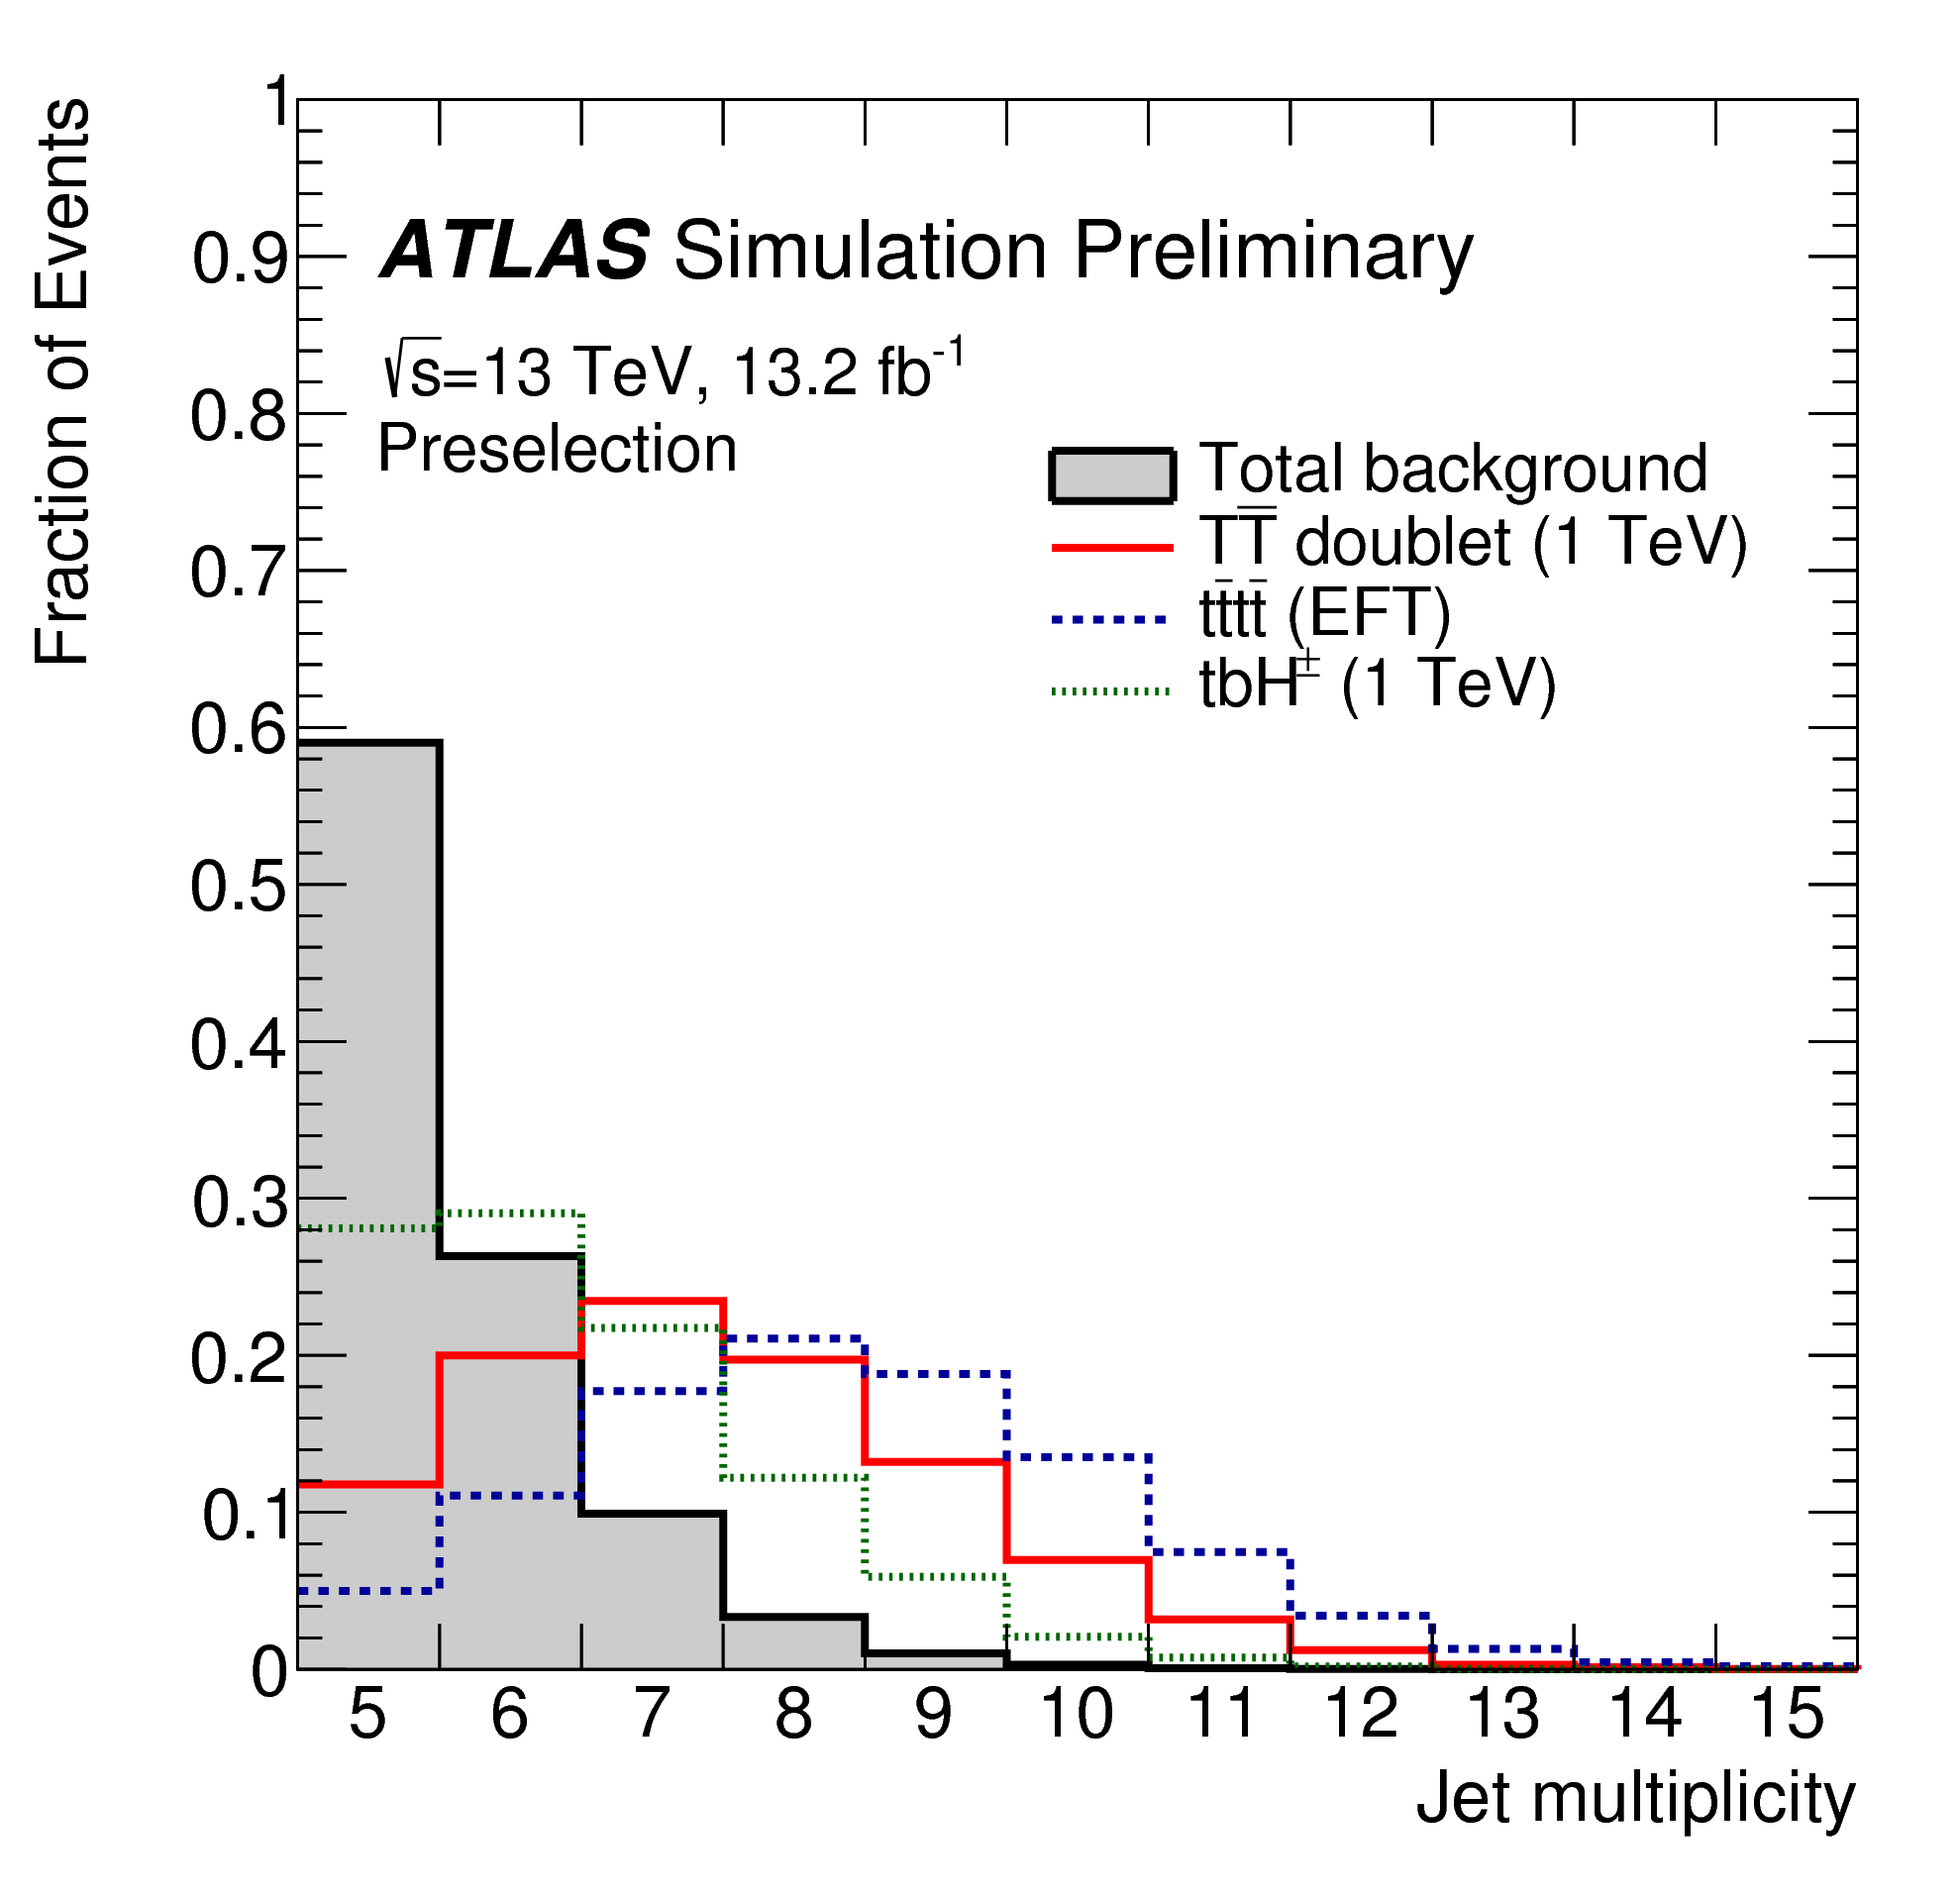
\includegraphics[width=0.9\textwidth]{figures/VLQ/njets.png}
  \caption{}
  \label{fig:vlq:str:njets}
\end{subfigure}
\begin{subfigure}{0.5\textwidth}
  \centering
  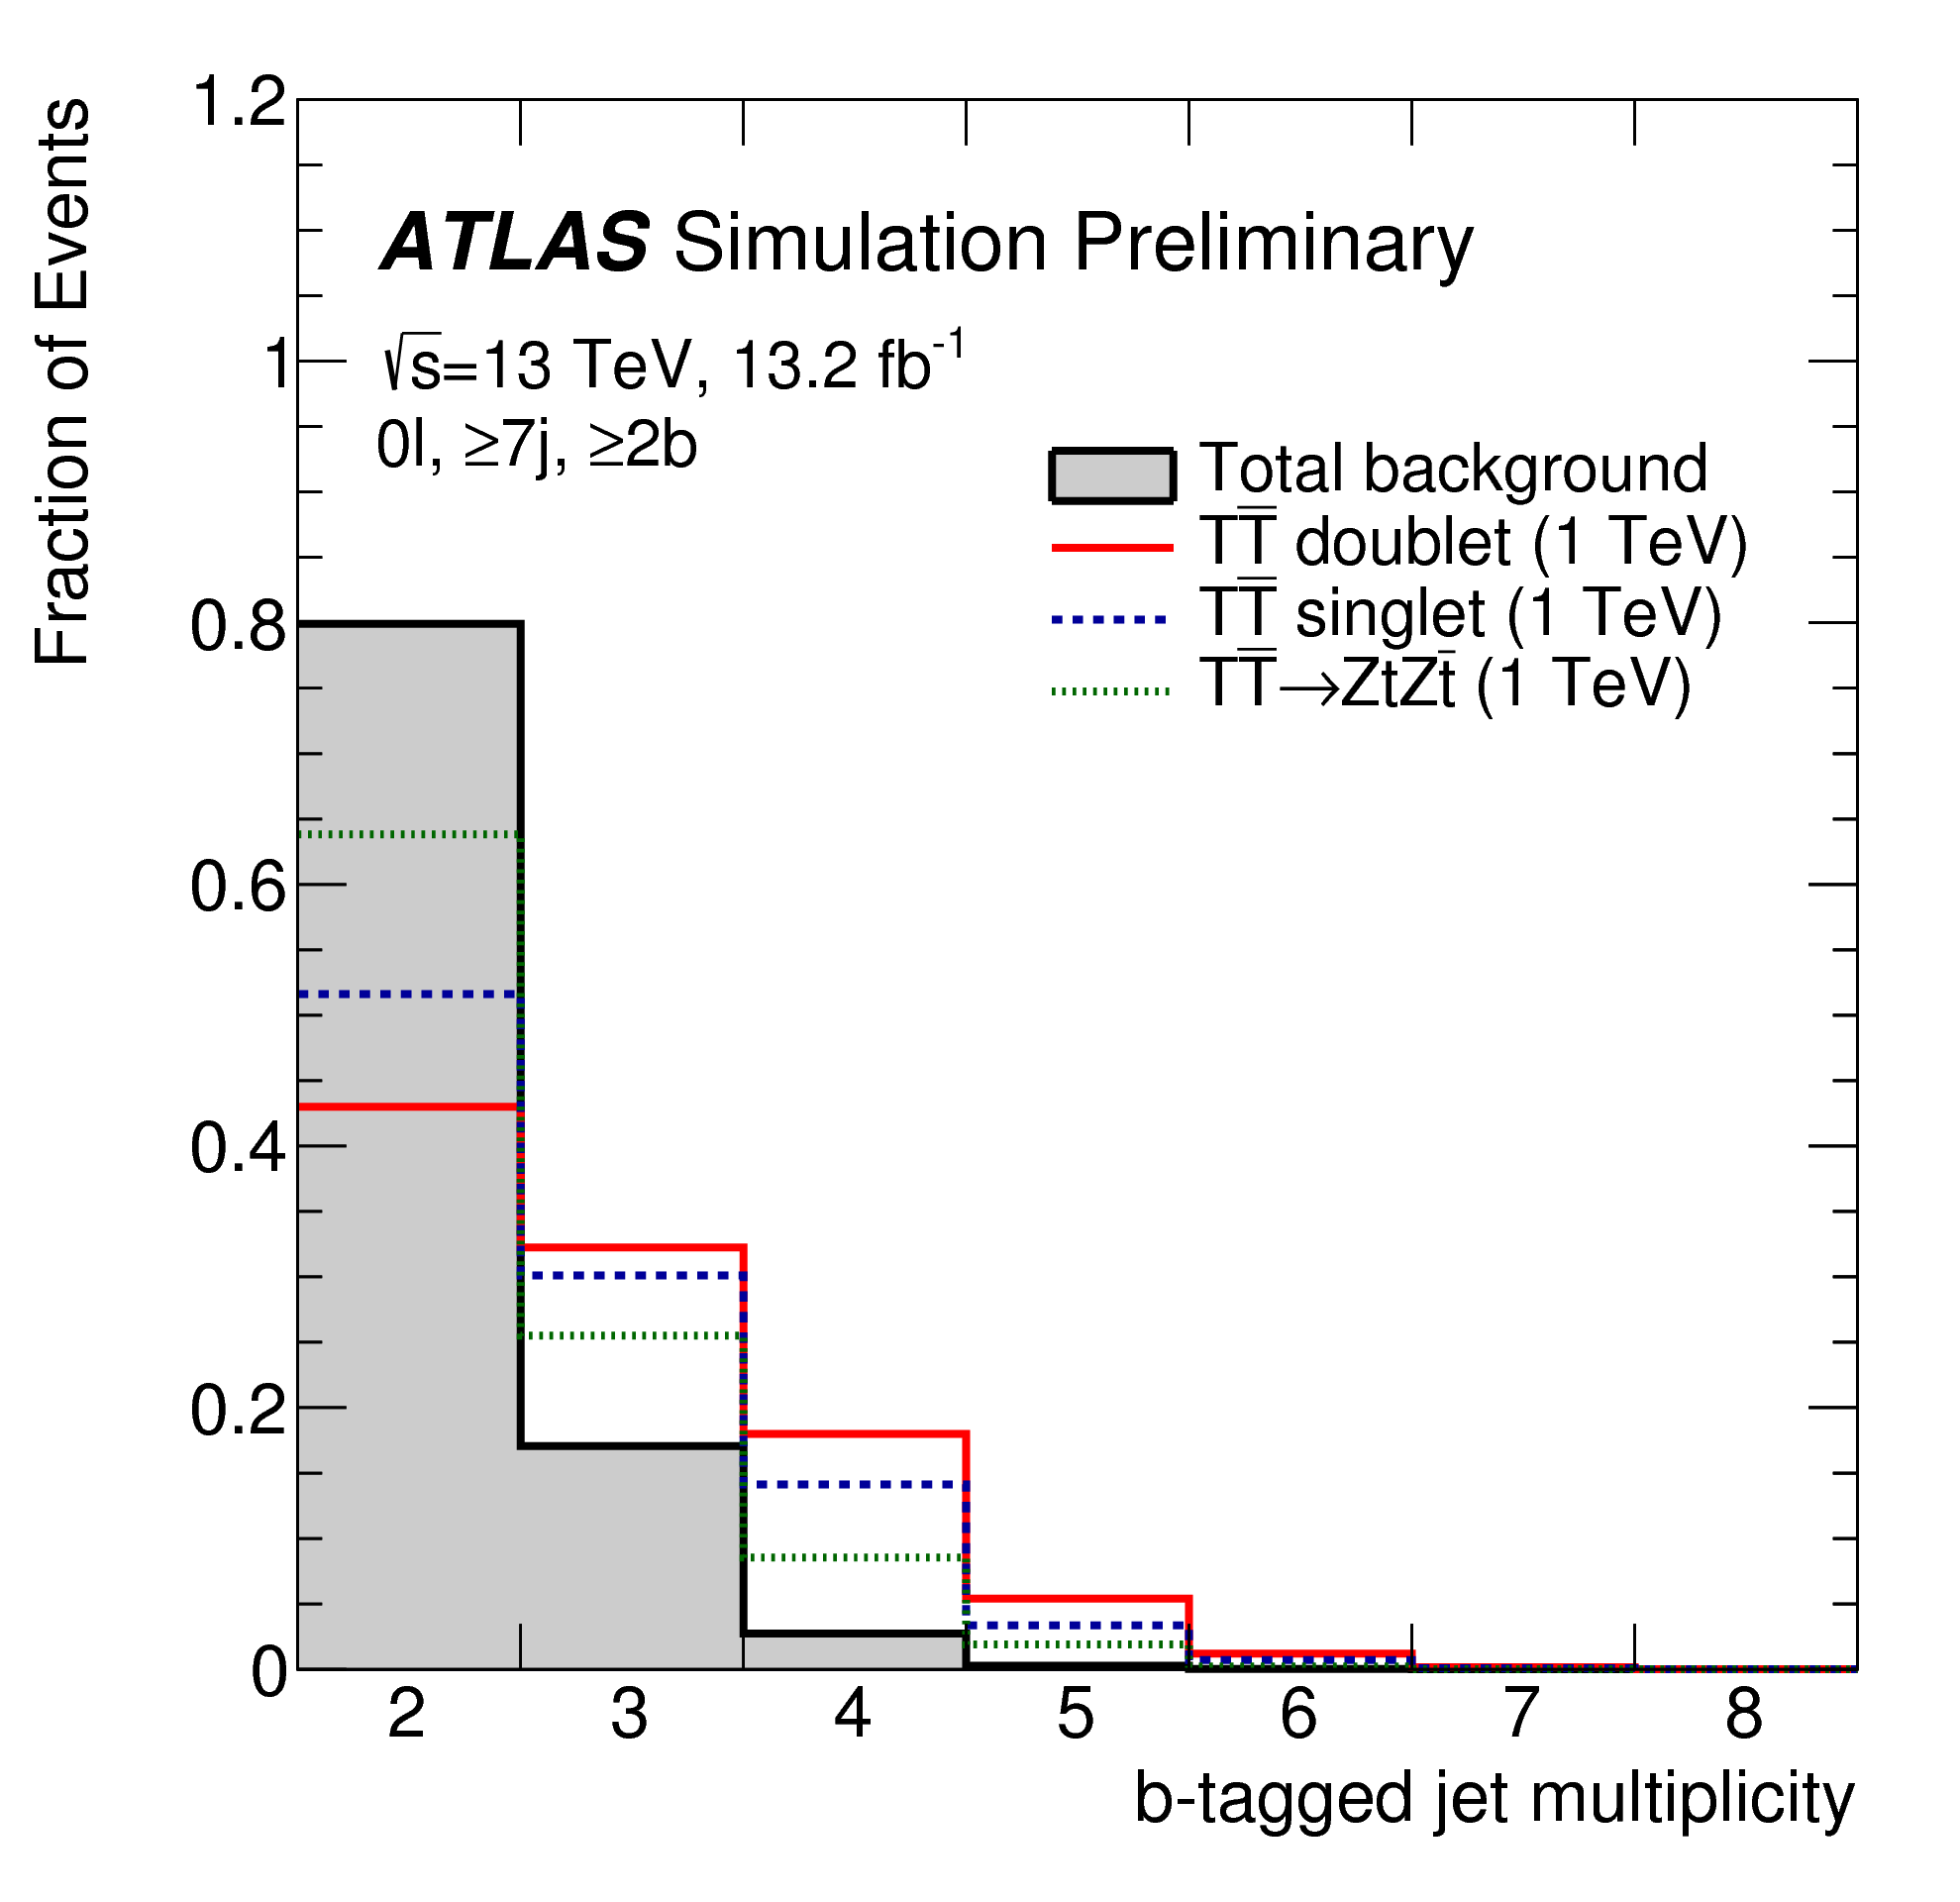
\includegraphics[width=0.9\textwidth]{figures/VLQ/nbjets.png}
  \caption{}
  \label{fig:vlq:str:nbjets}
\end{subfigure}

\captionsetup{width=0.85\textwidth} \caption{\small Comparison of the shape of (a) the jet multiplicity distribution in the 1-lepton channel after preselection, and (b) the $b$-tag multiplicity distribution in the 0-lepton channel after preselection plus the requirement of $\ge$7 jets, between the total background (shaded histogram) and several signal scenarios considered in this search. The signals shown are: $T\bar{T}$ production in the weak-isospin doublet and singlet scenarios, and for ${\rm BR}(T\to Zt) = 1$, assuming $m_{T} = 1$ \tev; $t\bar{t}t\bar{t}$ production within an EFT model; and $tbH^{\pm}(\to tb)$ production assuming $m_{H^{\pm}} = 1$ \tev. The last bin contains the overflow.}
\label{fig:vlq:str:jetmult}
\end{figure}
The increase of centre-of-mass energy in Run 2 gives the possibility to explore higher-mass signals compared to the ones accessible during Run 1. High-mass $T$ quarks may decay into boosted SM particles ($W$, $Z$, Higgs bosons and top quarks) potentially giving rise to high multiplicity of large-$R$ jets capturing their products, which can be used to further discriminate signal from background. Large-$R$ jets used in this search are RT-jets with $\pt> 300$ $\gev$, $|\eta|<2.0$ and mass above 100 \gev. The latter requirement is used to identify boosted top-quark and Higgs-boson candidates. Background $t\bar{t}$+jets events are expected, both in 1-lepton and 0-lepton channels, to contain up to one mass-tagged jet from a boosted, hadronically-decaying top quark, while signal events are characterised by higher mass-tagged jet multiplicity as shown in figure \ref{fig:vlq:str:hotmult}.\par 
\begin{figure}[h!]
\centering
\includegraphics[width=0.5\textwidth]{figures/VLQ/nHOT.png}

\captionsetup{width=0.85\textwidth} \caption{\small Comparison of the shape of the mass-tagged jet multiplicity distribution in the 0-lepton channel after preselection plus the requirement of $\ge$7 jets, between the total background (shaded histogram) and several signal scenarios considered in this search. The signals shown are: $T\bar{T}$ production in the weak-isospin doublet and singlet scenarios, and for ${\rm BR}(T\to Zt) = 1$, assuming $m_{T} = 1$ \tev. The last bin contains the overflow.}
\label{fig:vlq:str:hotmult}
\end{figure}
In order to optimise the sensitivity of the searches, the selected events are categorised into different regions depending on the jet multiplicity (5 and $\ge$6 jets in the 1-lepton channel; 6 and $\ge$7 jets in the 0-lepton channel), $b$-tag multiplicity (2, 3 and $\ge$4) and mass-tagged jet multiplicity (0, 1 and $\ge$2). In the following, channels with $N$ mass-tagged jets, $n$ jets, and $m$ b-tagged jets are denoted as ($N$J, $n$j, $m$b). In addition, events in particular regions are further categorised by exploiting the kinematic features of the signal and the background. In the case of the $T\bar{T}\to Ht+X$ signal, the presence of a partially-boosted Higgs boson is exploited using the property that the $b\bar{b}$ pair from the Higgs boson decay has smaller angular separation than pairs resulting from combinatorial background. In this regime, the two $b$-jets are separated enough as to be reconstructed in two individual jets but are very close in $\Delta R$. The mass of the $b\bar{b}$ pair with smallest $\Delta R$ distance, $m_{b\bar{b}}^{{\rm min}\Delta R}$ , provides a good approximation to the reconstructed $H \to b\bar{b}$ invariant mass, as shown in figure \ref{fig:vlq:str:mbbmin} for events in the (1J, $\ge$6j, $\ge$4b) region of the 1-lepton channel.
This distribution, which for signal shows a clear peak near 125 \gev, allows the classification of events into two regions depleted or enriched in $T\to Ht,H\to b\bar{b}$ decays, by requiring $m_{b\bar{b}}^{{\rm min}\Delta R}<$ 100 $\gev$ (referred to as ``LM'', standing for ``low mass'') or $m_{b\bar{b}}^{{\rm min}\Delta R}>$  100 $\gev$ (referred to as ``HM'', standing for ``high mass''). 
The minimum transverse mass between \MET and any of the three leading $b$-tagged jets in the event, $m_{\rm T,min}^b$, is used instead in the 0-lepton channel. This variable exhibits excellent separation between signal and background, which shows a Jacobian peak around the top quark mass, as shown in figure \ref{fig:vlq:str:mtbmin} for events in the ($\ge$2J, $\ge$7j, $\ge$3b) region of the 0-lepton channel. Therefore, two regions are defined: $m_{\rm T,min}^b>$ 160 $\gev$ (referred to as ``LM'', standing for ``low mass'') and $m_{\rm T,min}^b<$ 160 $\gev$ (referred to as ``HM'', standing for ``high mass''), the latter having a higher signal-to-background ratio than the former.


\begin{figure}[h!]
\begin{subfigure}{0.5\textwidth}
  \centering
  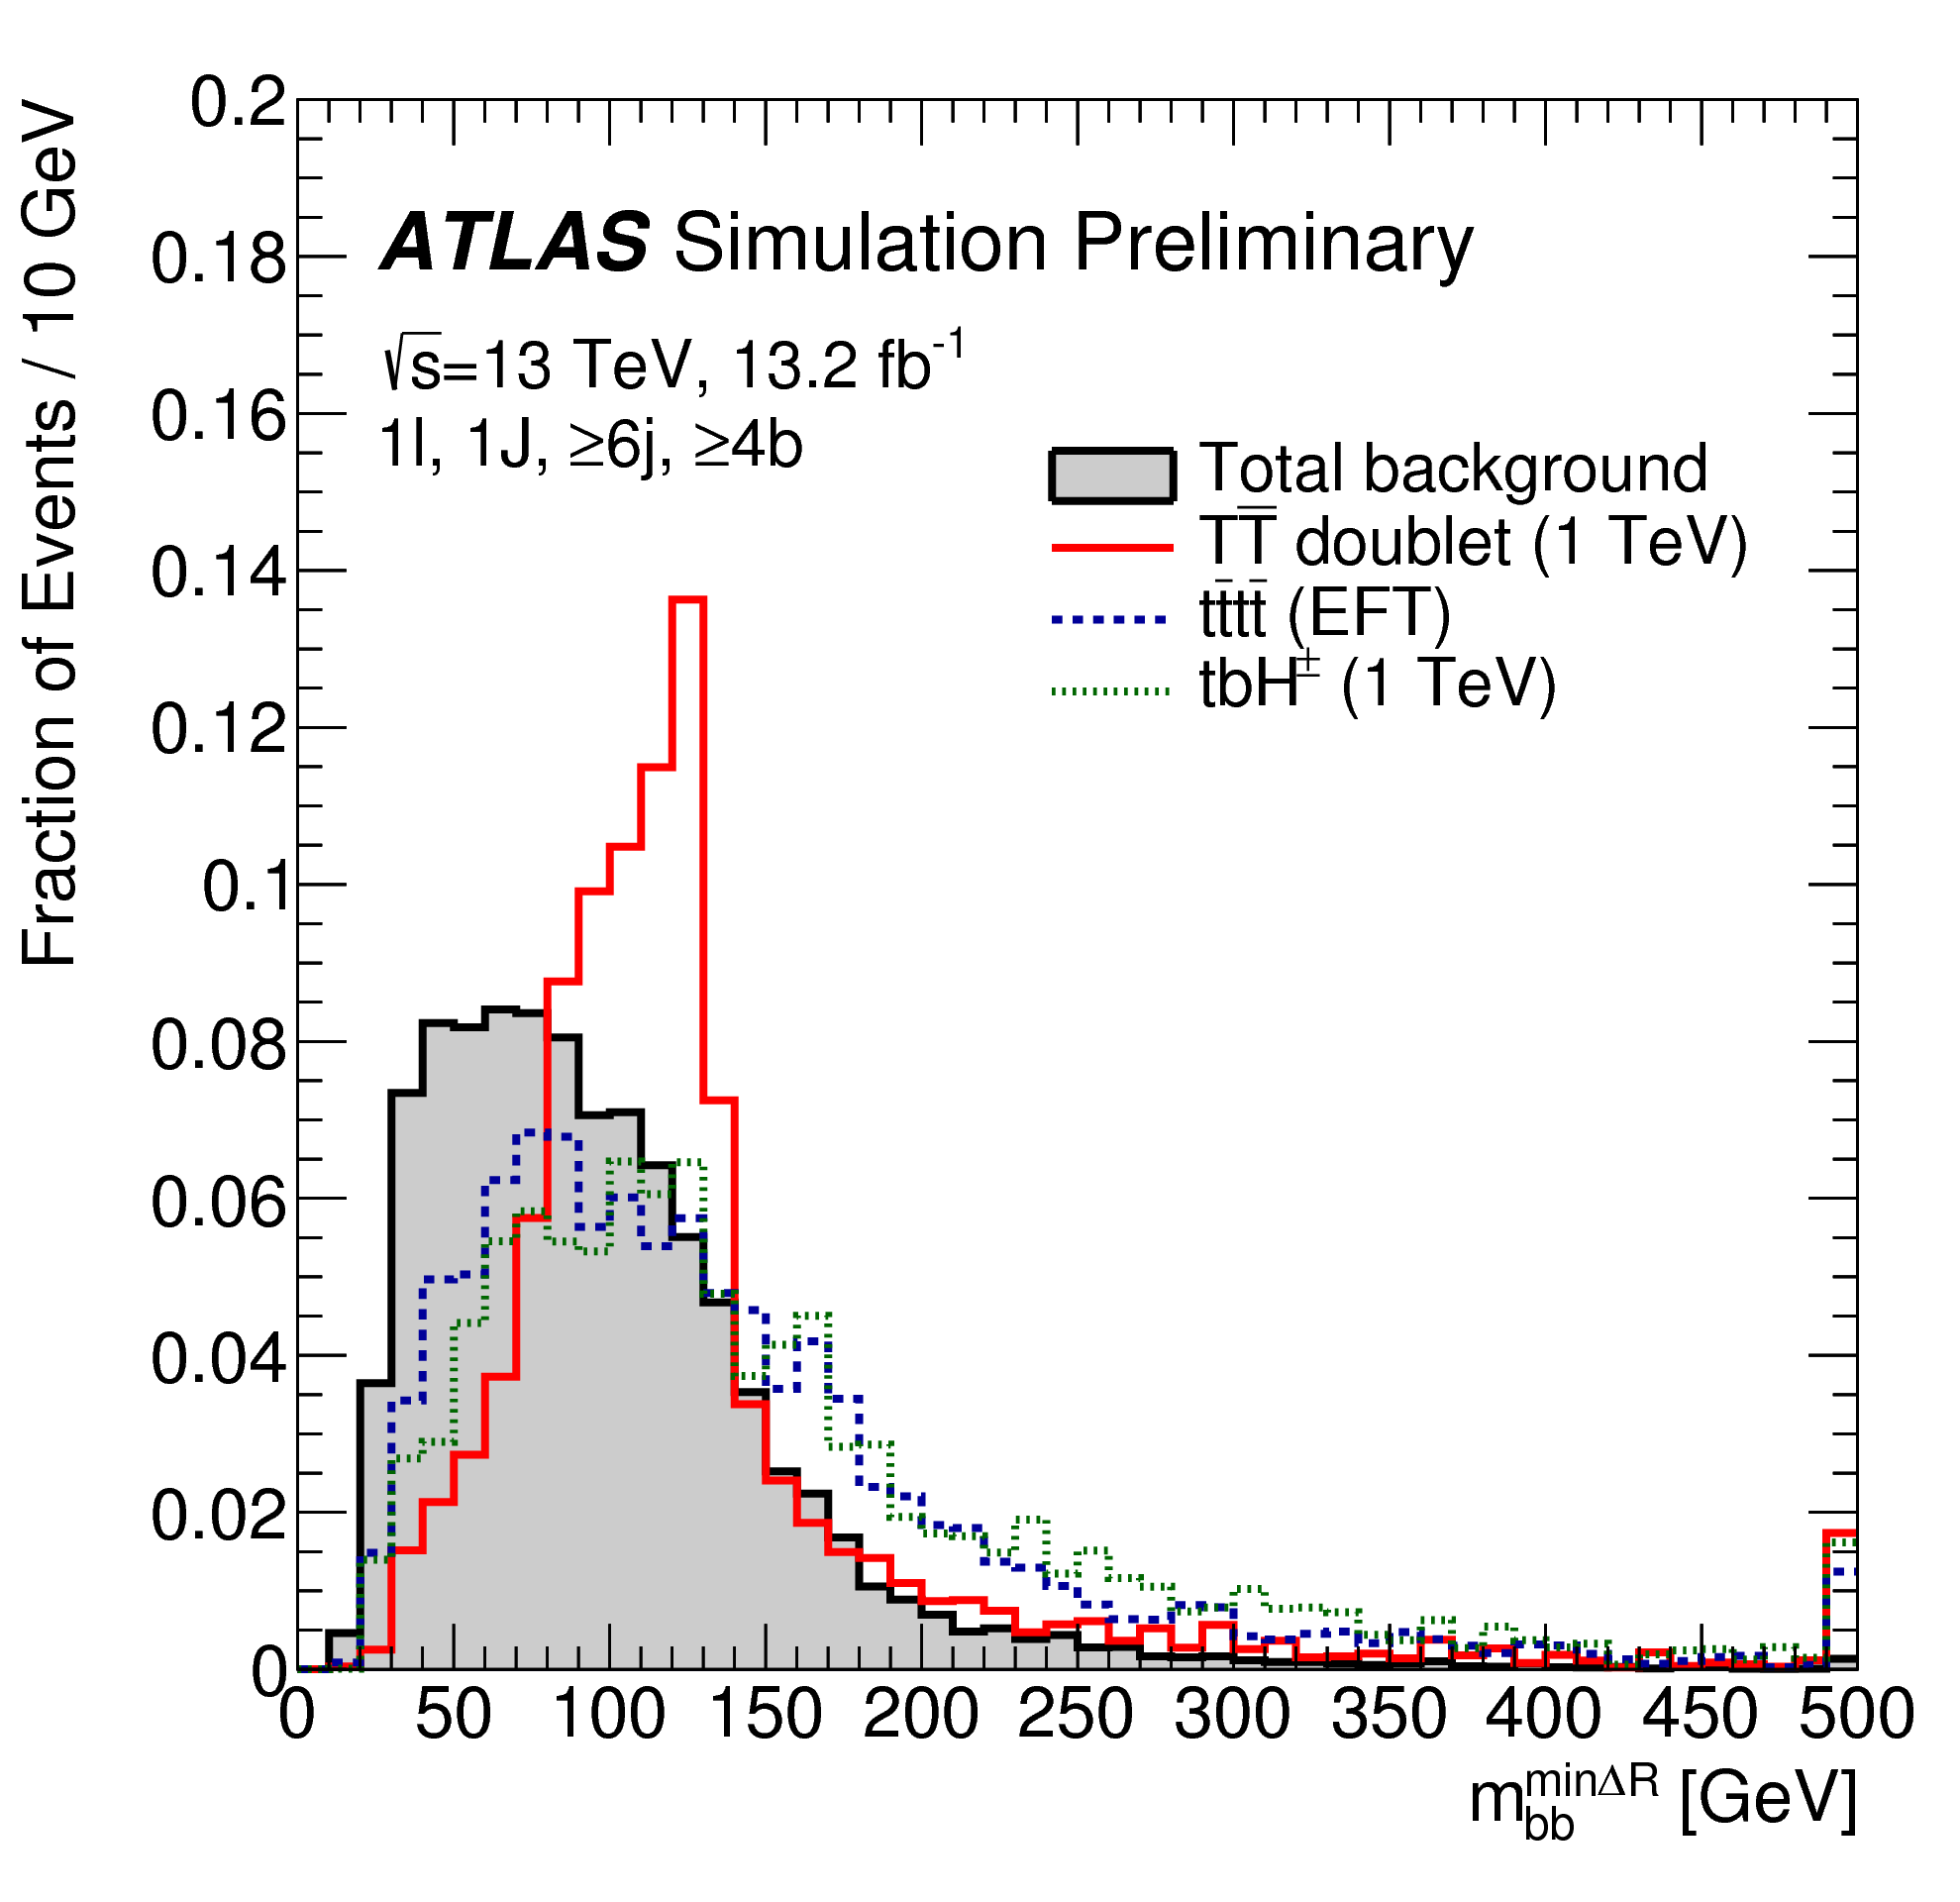
\includegraphics[width=0.9\textwidth]{figures/VLQ/mbb.png}
  \caption{}
  \label{fig:vlq:str:mbbmin}
\end{subfigure}
\begin{subfigure}{0.5\textwidth}
  \centering
  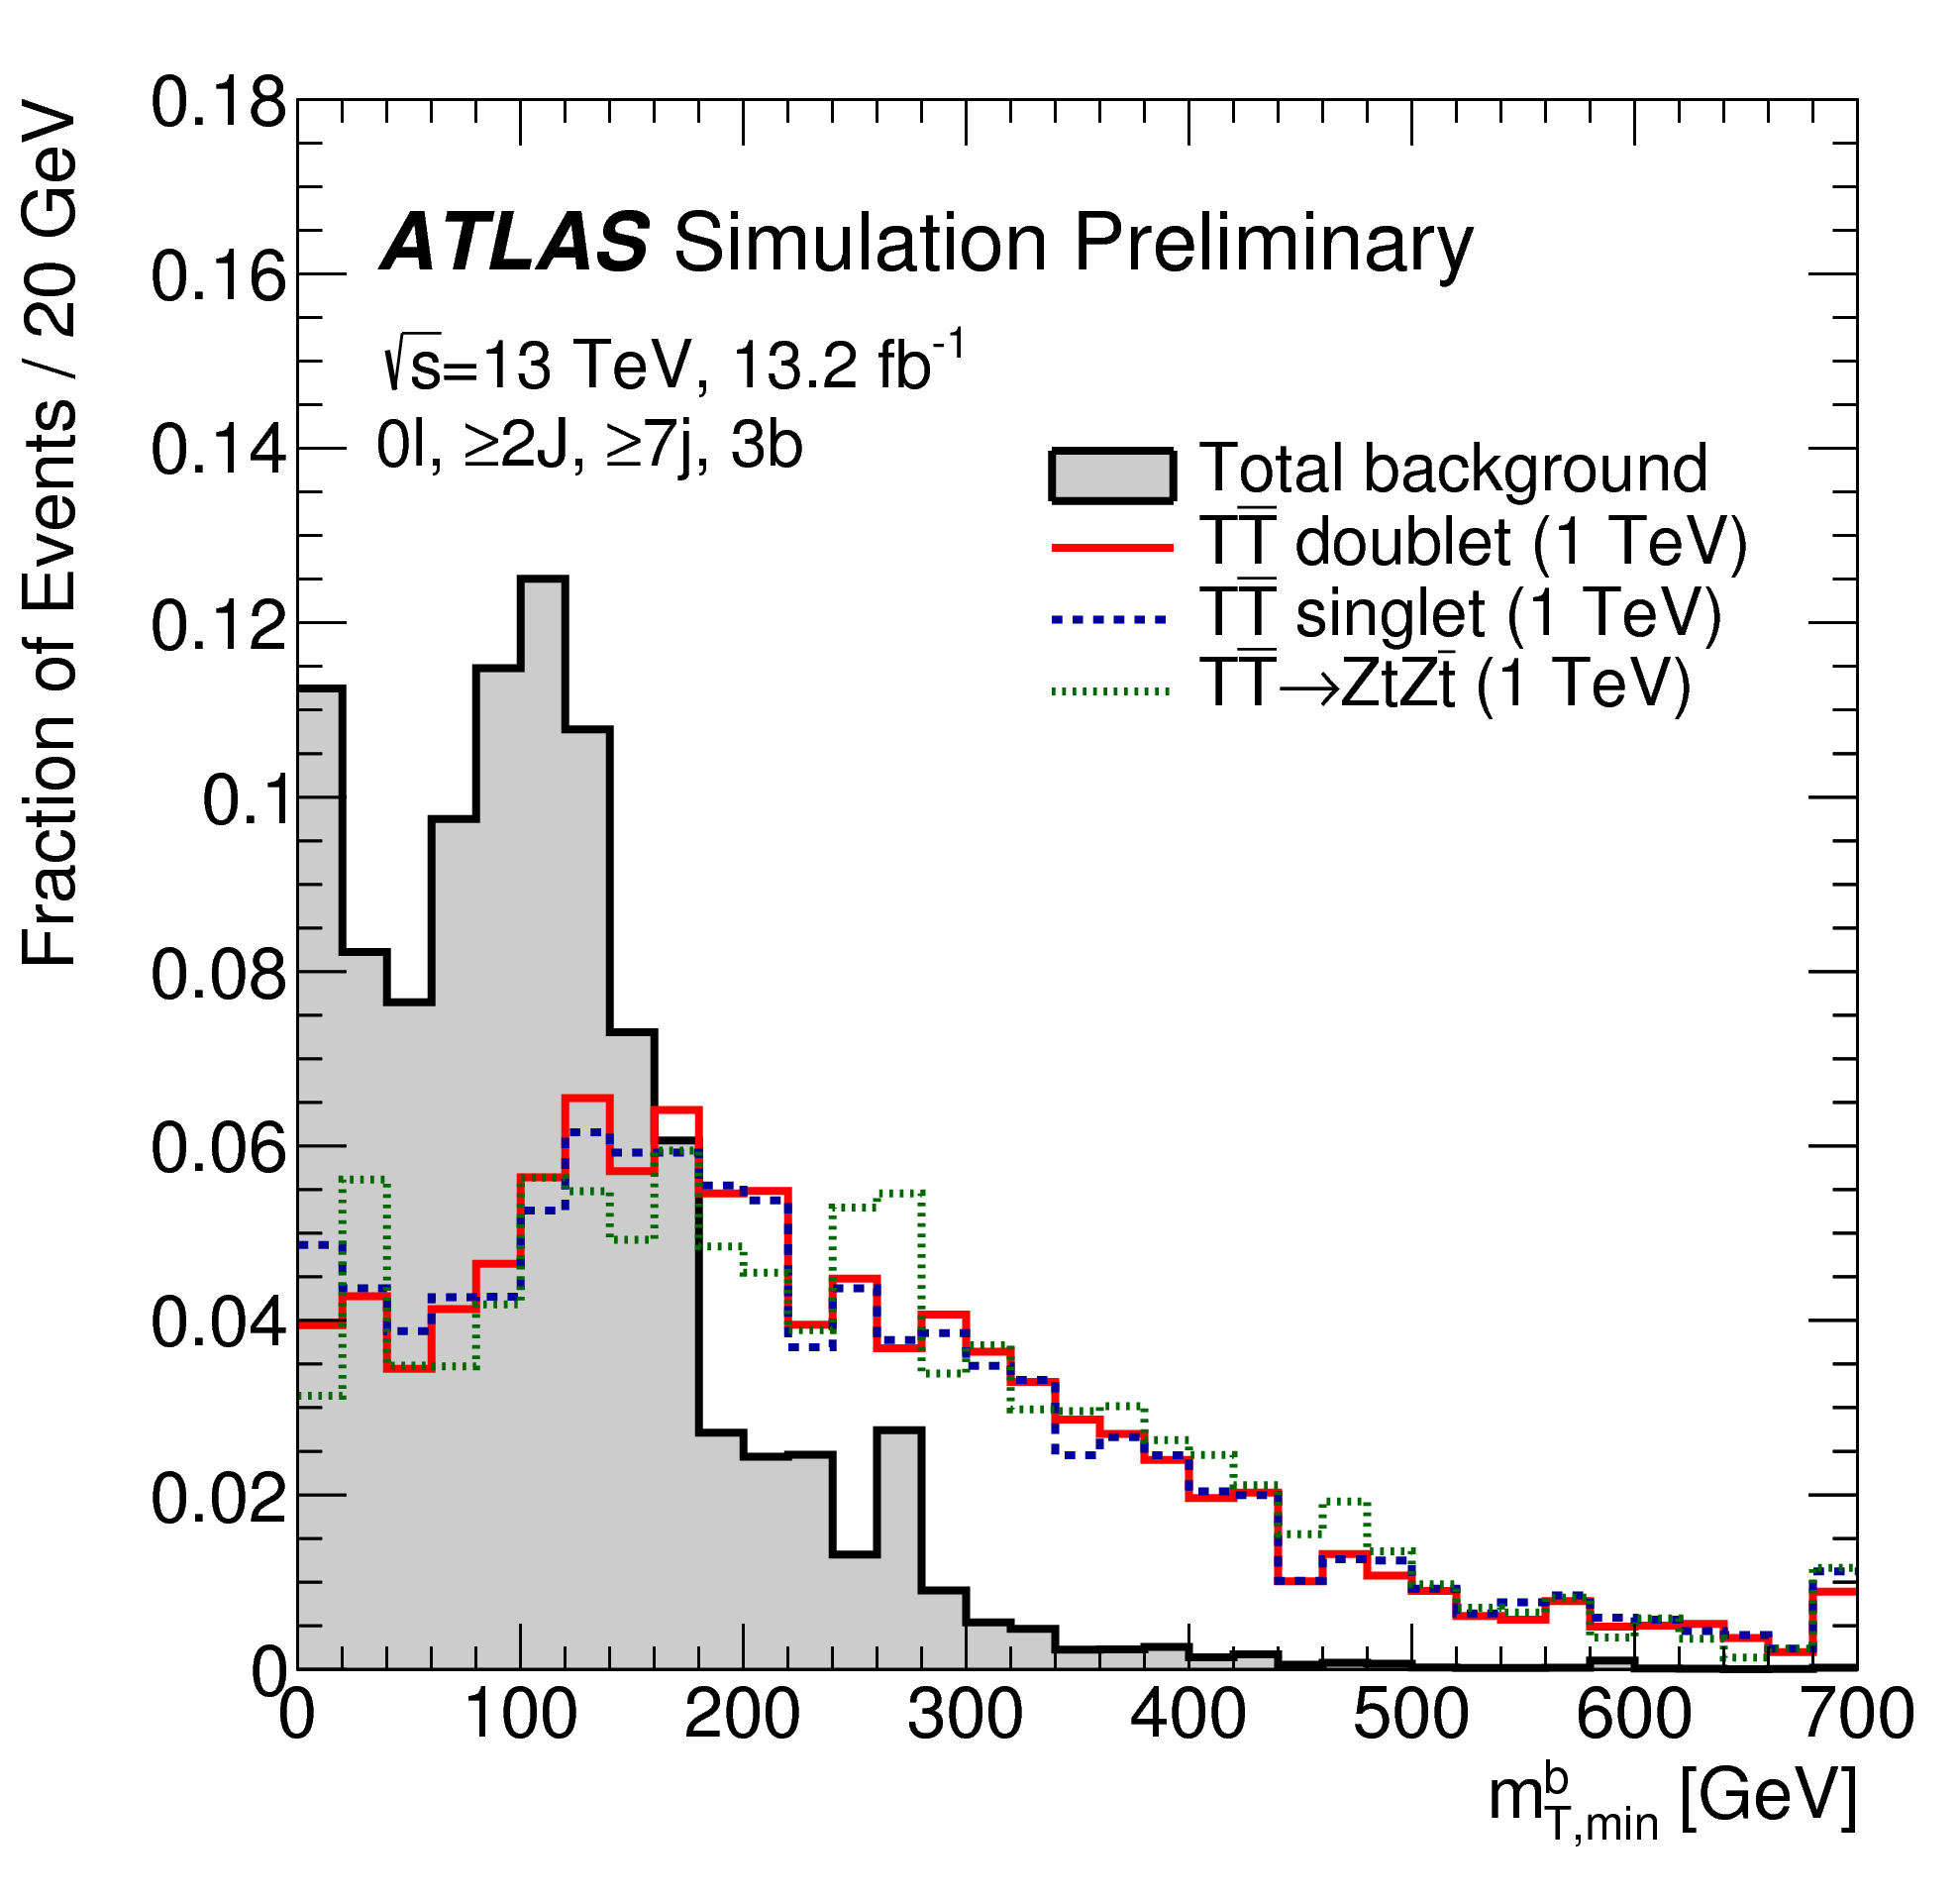
\includegraphics[width=0.9\textwidth]{figures/VLQ/mtbmin.png}
  \caption{}
  \label{fig:vlq:str:mtbmin}
\end{subfigure}

\captionsetup{width=0.85\textwidth} \caption{\small Comparison of the shape of (a) the invariant mass distribution of the two $b$-tagged jets with lowest $\Delta$R separation ($m_{b\bar{b}}^{{\rm min}\Delta R}$), and (b) the distribution of the minimum transverse mass between \MET and any of the three leading $b$-tagged jets in the event ($m_{\rm T,min}^b$), between the total background (shaded histogram) and several signal scenarios considered in this search. The signals shown are: $T\bar{T}$ production in the weak-isospin doublet and singlet scenarios, and for ${\rm BR}(T\to Zt) = 1$, assuming $m_{T} = 1$ \tev; $t\bar{t}t\bar{t}$ production within an EFT model; and $tbH^{\pm}(\to tb)$ production assuming $m_{H^{\pm}} = 1$ \tev. The selection used in (a) corresponds to events in the (1J, $\ge$6j, $\ge$4b) region of the 1-lepton channel, whereas the selection used in (b) corresponds to events in the ($\ge$2J, $\ge$7j, 3b) region of the 0-lepton channel. The last bin contains the overflow.}
\label{fig:vlq:str:addvar}
\end{figure}

